%!TeX root=../tese.tex
%("dica" para o editor de texto: este arquivo é parte de um documento maior)
% para saber mais: https://tex.stackexchange.com/q/78101/183146

%% ------------------------------------------------------------------------- %%
\chapter{Plataforma de Desenvolvimento}
\label{cap:plataforma de desenvolvimento}
\section{Estrutura Básica}

Quando se trata de desenvolvimento de jogos, o conceito de programação não pode se limitar aos tipos de programa \textquotedbl{\textit{batch mode}}\textquotedbl{}, isso é, programas que são executados em apenas duas etapas: o programador executa o programa; o programa devolve um resultado~\citep{IAEmTowerDefense}. Esse modelo é frequentemente usado, ainda mesmo nos dias atuais, para processamento de grandes volumes de dados, suportar reprodutibilidade, flexibilidade em termos de momento de execução, e geração de logs detalhados, entre outros cenários~\citep{BatchProgramming}.

Os programas interativos, por sua vez, compõem a estrutura dos jogos digitais como conhecidos atualmente. Este modelo, por sua vez, se resume ao pequeno bloco de código a seguir.

\begin{program}
    \lstinputlisting[language=Python, style=wider]
    {conteudo/gameloop.py}
  
    \caption{Game Loop\label{prog:gameloop}.}
\end{program}

Essa estrutura é conhecida como \textit{Game Loop}~\citep{GameProgramming}. O jogo primeiramente processa o input recebido pelo usuário, atualiza as variáveis do jogo de acordo e, finalmente, desenha os resultados na tela. Este pequeno trecho de código é projetado para ser executado, idealmente, um total de 60 vezes por segundo, em intervalos de tempos iguais, gerando a denominada \textit{frame}\footnote{
    Um \textquotedbl{quadro}\textquotedbl{} do jogo. A rápida sequência de quadros gerados pelo \textit{game loop} resulta na animação geral do jogo.
}. Com isso, cada \textit{frame} do jogo será apresentada apenas durante aproximadamente 0.016 segundos até ser substituída pela próxima pelo código do \textit{Game Loop}.

Por uma questão de simplicidade e para eliminar a necessidade de recriar essa estrutura para qualquer programa interativo, \textit{frameworks} dedicadas para o desenvolvimento desse tipo de programa tornaram-se disponíveis, mais especificamente para o cenário de desenvolvimento de jogos, as \textit{Game Engines}\footnote{
    Alguns exemplos de \textit{engines} famosas hoje em dia: Unity; Unreal Engine; CryEngine; GameMaker Studio; RPG Maker; Godot.
}. Também conhecidas como \textit{Motor de Jogo}, essas auxiliam fortemente no desenvolvimento tanto jogos 2D quanto 3D, além de uso de gráficos, audio, bancos de dados, físicas, ou até mesmo uso de outras \textit{frameworks} para, por exemplo, comunicação entre redes. A \textit{engine} utilizada para desenvolver o protótipo neste estudo foi a \textit{Godot Engine}.

\section{Funcionalidades e Aplicações da Godot}

A \textit{Godot Engine} é uma \textit{engine} totalmente gratuita e \textit{open-source} sob a licença MIT, dedicada para o desenvolvimento de aplicativos 2D ou 3D, principalmente jogos eletrônicos, e tem sua manutenção feita atualmente pela comunidade de forma independente. A versão da engine utilizada neste estudo foi a 3.2.3, parte da versão 3.0 da \textit{Godot}, lançada em 2018. Para entendimento do protótipo desenvolvido e do estudo feito, esta seção será dedicada a explicar os elementos básicos da \textit{engine}, assim como algumas funcionalidades adicionais.

Falar esse finalzinho? numsei

\subsection{Nós}

Também conhecidos como \textit{Nodes}, quando separados, representam pequenos elementos do jogo. Quando juntos, compoem a estrutura geral do jogo, como blocos de construção. Na \textit{Godot}, exitem diversos tipos diferentes de nós, cada um com uma função específica, e possivelmente herdando funcionalidades de outros tipos de nós. Por outro lado, os nós terão por padrão as seguintes utilidades:

\begin{itemize}
    \item Possuem um nome;
    \item Possuem atributos (variáveis);
    \item Podem possuir ou não um trecho de código que é chamado toda \textit{frame} do jogo, definido em um \textit{script};
    \item Podem possuir ou não métodos customizados, definidos no \textit{script} mencionado;
    \item Podem herdar funcionalidades de outros nós ou scripts criados;
    %(tendo assim atributos e métodos de ambos scripts, o atribuído e o herdado)
    \item Podem ser inseridos como \textit{filhos} de outros nós, compondo uma \textit{cena}.
    %, herdando \textquotedbl{forçadamente}\textquotedbl{} atributos como posição na tela
\end{itemize}

Usufruindo de todas essas funções, o desenvolvimento do jogo é focado quase totalmente no uso dos nós.

\begin{figure}
    \centering

    \begin{subfigure}{.9\textwidth}
        \centering
        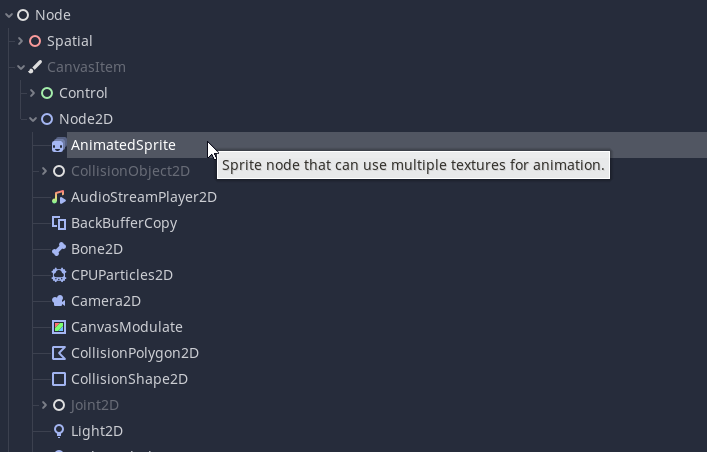
\includegraphics[width=1\textwidth]{tiposDeNos}
    \end{subfigure}

    \caption{Tela de criação de \textit{novo nó}, dentro da \textit{Godot}.}
\end{figure}

\subsection{Cenas}

Como mencionado anteriormente em~\ref{Cenas}, uma cena pode representar tanto um estado específico do jogo, por exemplo uma fase, como um determinado \textquotedbl{objeto}\textquotedbl{}, por exemplo, o personagem principal ou um inimigo. Cenas são sempre compostas por um ou mais nós em uma estrutura hierárquica. O editor da \textit{Godot} possui uma seção intuitiva para criação e modificação dessa hierarquia, como demonstrado a seguir.

\begin{figure}
    \centering

    \begin{subfigure}{.4\textwidth}
        \centering
        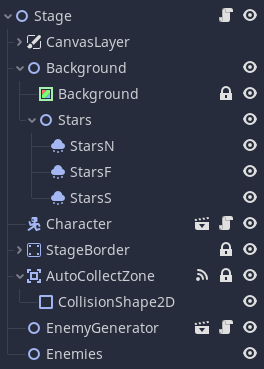
\includegraphics[width=1\textwidth]{arvoreDeNos}
    \end{subfigure}

    \caption{Árvore de nós da cena/fase principal do jogo.}
\end{figure}

O nó principal \textit{Stage} está no topo da hierarquia da cena, portanto este controlará alguns dos atributos de seus nós \textquotedbl{filhos}\textquotedbl{}, como sua posição na tela. Isso é, a posição absoluta de um nó será sempre a soma vetorial de sua própria posição e a posição de seu nó \textquotedbl{pai}\textquotedbl{}.

Ao executar o jogo, significa que uma cena é executada. É possível executar a cena do personagem principal sem ela estar sendo instanciada em nenhuma outra cena. No protótipo criado, porém, sempre será executada uma cena de fase (ou \textit{Stage}) contendo tal personagem, assim tornam-se possíveis as interações entre os ataques e movimentos do personagem com o cenário, inimigos e itens. Com isso, cenas provam-se úteis para, principalmente, organização do projeto e uso de \textit{instanciação}.

\subsection{Instanciação}

Ao estruturar uma cena, esta pode ser tratada como uma classe e ser instanciada como um objeto para fazer parte da hierarquia de qualquer outra cena, assim como nós simples. Isso provou-se extremamente útil no desenvolvimento do protótipo em questão para, por exemplo, geração de projéteis. Com o alto número de projéteis ativos em \textit{Shmups} no geral, basta definir um projétil simples e instanciá-lo diversas vezes na posição do personagem ou do inimigo para gerar um cenário simples de combate.

A depender do cenário em que uma cena é instanciada, porém, torna-se necessário carregá-la previamente através de um \textit{script}, para possibilitar sua instanciação sob demanda, por exemplo, do \textit{input}\footnote{
    Qualquer ação, parametrizada no jogo, vinda do jogador, como um clique do mouse, ou uma tecla apertada no teclado.
} do jogador. Este processo é feito frequentemente na definição de inimigos e do personagem no protótipo.

\subsection{Sinais}

Para que nós e cenas possam detectar ocorrência de eventos fora de sua própria hierarquia, a \textit{Godot} disponibiliza um sistema de emissão e recepção de sinais. Um sinal pode ser emitido por um nó e recebido por um ou mais outros nós ou cenas, acionando assim, um método determinado na configuração do sinal. Muitos nós possuem sinais pré definidos, porém é possível criar sinais customizados através do \textit{script} da cena. Sinais provam-se convenientes para checagem de colisão de qualquer tipo. Por exemplo, quando um nó do tipo \textit{Area2D} intercala seu corpo com algum outro nó \textit{KinematicBody2D}\footnote{
    Nó principal do personagem, este possuindo métodos úteis de física para controle de movimento.
}, \textit{StaticBody2D} ou \textit{RigidBody2D}, este dispara um sinal de \textit{Body Entered}, configurado para tratar a colisão destes dois corpos. Um exemplo mais concreto seria um tiro do personagem entrando em contato com um inimigo, e este, com isso, executando seu método de \textit{receber dano}.

\subsection{Grupos}\label{Grupos}

Para um melhor desempenho na checagem de colisões, objetos que podem colidir com outros podem ser adicionados a grupos. Após definir a qual grupo um objeto pertence, é necessário também definir com quais grupos o objeto pode interagir. A figura a seguir mostra o grupo do personagem principal e seus grupos interagíveis.

\begin{figure}
    \centering
  
    \begin{subfigure}{0.4\textwidth}
        \centering
            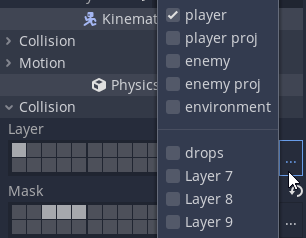
\includegraphics[width=.9\textwidth]{playerGroup}
        \caption{Grupo ao qual o personagem faz parte (\textit{Layer}).}
    \end{subfigure}
    % ATENÇÃO: Se você deixar uma linha em branco entre as subfiguras,
    % LaTeX vai considerar que cada uma delas pertence a um "parágrafo"
    % diferente e, portanto, vai colocá-las em linhas separadas ao invés
    % de lado a lado.
    \begin{subfigure}{0.4\textwidth}
        \centering
            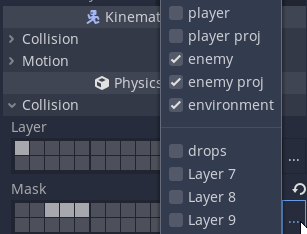
\includegraphics[width=.9\textwidth]{playerCollidable}
        \caption{Grupos com os quais o personagem pode interagir (\textit{Mask}).}
    \end{subfigure}
  
    \caption{Uso de grupos para colisão do personagem.}
\end{figure}

Isso é, o personagem poderá interagir apenas com objetos pertencentes aos grupo \textit{enemy}, \textit{enemy proj} e \textit{environment}, e com isso, colisões com outros grupos serão ignoradas. Este tipo de arquitetura contribui para a otimização geral do jogo ao não permitir que projéteis interajam com outros do mesmo tipo. Assim, centenas de checagens de colisão por segundo são poupadas, liberando tempo de processamento para outros cálculos.

\subsection{Herança}

Ao definir classes customizadas a partir de \textit{scripts}, é possível fazer com que outras cenas herdem (extendam) tanto classes padrão da \textit{Godot} quanto o \textit{script} criado, dando acesso a métodos e atributos da classe herdada. Cenas como os diferentes níveis de projéteis do jogador herdam a classe base de \textquotedbl{projétil}\textquotedbl{}. Nela, são definidos métodos de movimento básico do projétil, tratamento de colisão e atributos básicos como velocidade, direção e dano. Cálculos mais avançados e específicos do personagem são feitos em classes mais abaixo na herança.

\subsection{Singletons}\label{sec:Singletons}

Com o uso de \textit{Singletons} é possível ter acesso globalmente a métodos e variáveis definidas no nessa classe, por qualquer outro \textit{script}. Similarmente ao uso de sinais, o uso de \textit{Singletons} permite uma rápida e simples comunicação entre cenas distintas. O código \ref{prog:main_nodes_getter}, usado no protótipo em muitas cenas, auxilia, por meio de \textit{setters} e \textit{getters}, o acesso às cenas do personagem, fase principal, e \textit{stats}, uma cena utilizada durante o desenvolvimento, dedicada a expor de variáveis na tela, como número de vidas, bombas, número de balas ativas e outras variáveis utilizadas no cálculo da dificuldade.

\subsection{Banco de Dados}

Não sendo obrigatório no desenvolvimento de jogos, porém, o uso de um banco de dados facilita na definição e na variação de diferentes objetos. No protótipo desenvolvido, esses objetos foram, principalmente, as fases e os inimigos. Como a \textit{Godot} não inicializa projetos por padrão com bancos de dados, foi utilizado um outro \textit{Singleton} (\ref{prog:db_manager}) a fim de criar um gerenciador simples de banco de dados para uso interno no jogo, com foco na recuperação de dados. Para definição de fases e ondas (\ref{ONDASNOMAR}), assim como padrões de ataques de inimigos, foram utilizados arquivos \textit{JSON}, os quais são recuperados utilizando as funções do singleton em questão e, em seguida, utilizados na instanciação de cenas sob demanda.

\subsection{Linguagem de Programação}

\textit{GDScript}, a principal linguagem utilizada na \textit{Godot}, é uma linguagem de programação de tipagem dinâmica de alto nível, muito semelhante a \textit{Python} e \textit{Lua}. A linguagem é otimizada para integrar com a \textit{engine}, além de ser simples e elegante, como as linguagens nas quais é inspirada. O uso da linguagem junto à \textit{Godot} possui diversas vantagens, entre elas:

\begin{itemize}
    \item É compilada rapidamente pela própria \textit{engine};
    \item Possui diversas classes úteis para criação de jogos, como vetores 2D e 3D, matrizes e diversas funções de álgebra linear, classes de \textit{Object} (a qual inclui nós) e identificadores de caminho de nós e \textit{Resources}\footnote{
        Arquivos do jogo, variando desde arquivos de \textit{scripts} até cenas, \textit{sprites} e vídeos.
    }, além de classes mais básicas, como listas e dicionários;
    \item Conversa dinamicamente com a interface da \textit{engine}, reconhecendo nós da cena atual, \textit{Singletons}, \textit{Resources}, entre outros elementos da interface;
    \item Suporte a trechos de código em C e C++ para otimização;
    \item Suporte para uso de múltiplas \textit{threads}.
\end{itemize}

Além disso, o editor possui diversas ferramentas dedicadas à depuração do código, permitindo o uso de \textit{breakpoints}, inspecionar o estado atual da execução, valores de variáveis, chamadas de funções e tempo de execução em cada uma delas, essa última sendo crucial para a etapa de otimização do jogo mencionada em \ref{Grupos}.